\subsection{The Product}\label{subsec:theProduct}
The research in this paper has culminated in a software product that allows a user to enter a timed regular expression (TRE), and have it converted into a timed automaton (TA).
We have named this piece of software "TREAT", short for "Timed Regular Expression to Automaton Transformation".
An overview of the data flow through the program, is shown in \cref{fig:TREATdiagram}.

%The following diagram shows the flow of data through the TREAT program. The diagram is meant as an overall outline, and is not supposed to be precise. 
\scalebox{0.9}{
    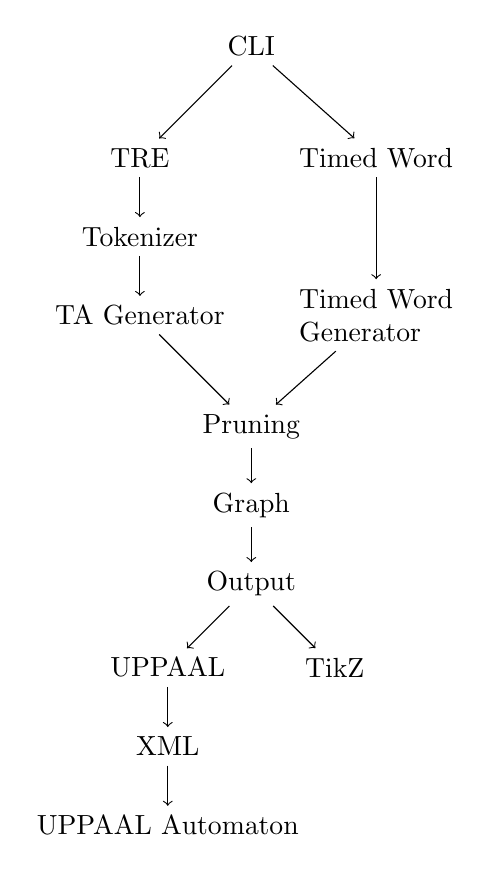
\begin{tikzpicture}[node distance = 1cm, auto]\label{fig:TREATdiagram}
        \node (CLI) {CLI};
        
        \node (TRE) [node distance = 2cm, below left of = CLI] {TRE};
        \node (TimedWord) [node distance = 3cm, right of = TRE] {Timed Word};
        \node (Tokenizer) [below of = TRE] {Tokenizer};
        \node (TAGenerator) [below of = Tokenizer] {TA Generator};
        \node (Pruning) [node distance = 2cm, below right of = TAGenerator] {Pruning};
        \node (Graph) [below of = Pruning] {Graph};
        \node (Output) [below of = Graph] {Output};
        \node (UPPAAL) [node distance = 1.5cm, below left of = Output] {UPPAAL};
        \node (XML) [below of = UPPAAL] {XML};
        \node (UPPAALAutomaton) [below of = XML] {UPPAAL Automaton};
        \node (TikZ) [node distance = 1.5cm, below right of = Output] {TikZ};
        \node (TimedWordGenerator) [node distance = 3cm, right of = TAGenerator,  align=left] {Timed Word\\Generator};
    
        \draw[->] (CLI) -- (TRE);
        \draw[->] (TRE) -- (Tokenizer);
        \draw[->] (Tokenizer) -- (TAGenerator);
        \draw[->] (TAGenerator) -- (Pruning);
        \draw[->] (Pruning) -- (Graph);
        \draw[->] (Graph) -- (Output);
        \draw[->] (Output) -- (UPPAAL);
        \draw[->] (UPPAAL) -- (XML);
        \draw[->] (XML) -- (UPPAALAutomaton);
        \draw[->] (Output) -- (TikZ);
        \draw[->] (CLI) -- (TimedWord);
        \draw[->] (TimedWord) -- (TimedWordGenerator);
        \draw[->] (TimedWordGenerator) -- (Pruning);
    \end{tikzpicture}
}


TREAT is accessed through a command line interface(CLI)(see \cref*{fig:TREATdiagram}). The user can type in their TRE, along with a few options such as adding a timed word through a .csv file, turning off pruning, and silencing any warnings or info messages using "--quiet".
The user can also decide the output format of the TA at this point using "--format".

If the user opted to add a timed word, it is loaded from the .csv file, into two arrays. Each unique symbol in the word is added to the alphabet. This is shown as a separate branching to the right from CLI in \cref*{fig:TREATdiagram}
Looking at the left branch from CLI in \cref*{fig:TREATdiagram}, an automaton is created, that represents the timed word. This is required for checking the TRE with UPPAAL. This automaton has a transition for each of the symbols of the alphabet, and broadcasts its symbol on channels at the correct time. Checking is described further in \cref{subsec:checking}.

The TRE is parsed into tokens by a tokenizer. These tokens are connected as children of one another, to form an abstract syntax tree (AST). 

This AST is sent from the tokenizer, to the TA Generator, as illustrated in \cref*{fig:TREATdiagram}. The TA can be created using the rules from Eugene et al., with the modifications described in \cref{subsec:semantics}.

This is done by visiting each node in the tree, and generating states and edges in the TA, according to the rules. Three visitors go through the tree: One checks whether intervals on any given transition are valid. Another goes through the AST, to convert the iterator and the absorbed iterator into lower level components using union and iterator. The last visitor is responsible for implementing the rules of all other tokens.

At the next stage, the TA is pruned as described in \cref{subsec:pruning}. 
% The dataformat of the internal TA is an object containing hashsets and dictionaries corresponding to the sets of the tuples described in \cref{sec:preliminaries}. 
% This means that the code executed in the functions responsible for pruning, map very closely to the mathematical operations in \cref{sec:preliminaries}.

Since the TA is now in its final form with regards to states, transitions, and the guards associated with them, each state is now assigned a position based on the algorithm described in \cref{subsec:graph}.

Finally, the TA is output to one of the selected formats as described in \cref{subsec:formats}. The different output formats are represented with separate branches in \cref*{fig:TREATdiagram}.
